\documentclass[10pt,a4paper]{article}
\usepackage[utf8]{inputenc}
\usepackage[french]{babel}
\usepackage[T1]{fontenc}
\usepackage{amsmath,amsfonts,amssymb}
\usepackage[squaren, Gray, cdot]{SIunits}
\usepackage{tikz}
\usepackage{circuitikz}
\usepackage[left=2cm,right=2cm,top=2cm,bottom=2cm]{geometry}
\usepackage{url}

\tikzset{
xmin/.store in=\xmin, xmin/.default=-3, xmin=-3,
xmax/.store in=\xmax, xmax/.default=3, xmax=3,
ymin/.store in=\ymin, ymin/.default=-3, ymin=-3,
ymax/.store in=\ymax, ymax/.default=3, ymax=3,
}
% Commande qui trace la grille entre (xmin,ymin) et (xmax,ymax)
\newcommand {\grille}
{\draw[help lines] (\xmin,\ymin) grid (\xmax,\ymax);}
% Commande \axes
\newcommand {\axes} {
\draw[->] (\xmin,0) -- (\xmax,0);
\draw[->] (0,\ymin) -- (0,\ymax);
}
% Commande qui limite l'affichage à (xmin,ymin) et (xmax,ymax)
\newcommand {\fenetre}
{\clip (\xmin,\ymin) rectangle (\xmax,\ymax);} 
 
\begin{document}{\bf Cours d'electronique} 

\section{Circuit série et U=RI}
Dans un circuit la tension (U exprimée en \volt ) est égale à la résistance (R exprimée en \ohm) multiplié par l'intensité (I exprimée en \ampere) ce qui donne l'équation~\eqref{uri}
\begin{equation}
U=R*I
\label{uri}
\end{equation}

Remarque en série les résistances s'additionnent.

Prenons un circuit avec les résistances R1= 5 \ohm, R2= 20 \ohm, R3= 30 \ohm
\shorthandoff{:!}
\begin{figure}[h!]
  \begin{center}
    \begin{circuitikz}
      \draw (0,0)
      to[V,v=$U_q$] (0,2) % The voltage source
      to[R=$R_1$,v_<=$U_1$] (2,2) % R1
      to[R=$R_2$,v_<=$U_2$] (4,2) % R2
      to[R=$R_3$,v_<=$U_3$] (6,2) % R3
      to[short,i=$i$] (6,0)
      to[short] (0,0);
    \end{circuitikz}
    \caption{Circuit simple.}
  \end{center}
\end{figure}

Remarque en série les résistances s'additionnent.
\begin{align}
R_t &=R_1+R_2+R_3 \\
    &=5+20+30 \\
    &=55 \ohm
\end{align}

\begin{align}
I&=\frac{U}{R} \\
I&=\frac{12}{55} \\
I&=0,218 \ampere \\
\end{align}
La loi d'additivité des tensions se vérifie donc 
\begin{align}
U1&=5*0,218=1,09 \volt \\
U2&=20*0,218=4,36 \volt \\
U3&=30*0,218=6,54 \volt \\
U_q&=U1+U2+U3~=12 \volt
\end{align}

\pagebreak 

\section{Circuit Parellèle et Conductance}
La conductance est l'inverse de la résistance $ C= \frac{1}{Rt} $

\shorthandoff{:!}
\begin{figure}[h!]
  \begin{center}
    \begin{circuitikz}
      \draw (0,0)
      to[V,v=$U_q$] (0,5) % The voltage source
      to[short] (4,5)
      to[short,i_=$i_t$] (4,4)
      (4,4) to[short,i_=$i_1$] (3,4)
      to[short] (3,3)
      (4,4) to[short,i_=$i_2$] (5,4)
      to[short] (5,3)
      (3,3) to[R=$R_1$,v_<=$U_1$] (3,2) % R1
      to[short] (3,1)
      (5,3) to[R=$R_2$,v_<=$U_2$] (5,2) % R2
      to[short] (5,1)
      (3,1) to[short] (4,1)
      (5,1) to[short] (4,1)
      to[short] (4,0)
      to[short] (0,0);
    \end{circuitikz}
    \caption{Conductance d'un circuit parallèle.}
  \end{center}
\end{figure} 

R1 = 50 \ohm R2 = 30 \ohm

Pour ce circuit la conductance $ C = \frac{1}{R1}+\frac{1}{R2} = \frac{1}{50}+\frac{1}{30} = \frac{8}{150} $
Ce qui nous donne $R_t=\frac{150}{8} = 18,75 \ohm $ 

Ici on voit que la résistance totale de notre circuit parallèle est inférieur à la plus petite des résistances.

Si on calcule $i_1=\frac{U_1}{R_1}=\frac{12}{50}=0,24 \ampere $ $i_2=\frac{U_2}{R_2}=\frac{12}{30}=0,4 \ampere $

Si on compare a la résistance totale $I=\frac{12}{18,75}=0,64 \ampere$ nos deux intensités sont bien égales. 

\section{la Puissance}

La puissance P est exprimée en \watt elle se calcule à l'aide de la tension et de l'intensité utilisé par le circuit $P=U*I$.

\begin{figure}[h!]
  \begin{center}    
    \begin{circuitikz}
      \draw (0,0)
      to[V,v=$U_g$] (0,2) % The voltage source
      to[R=$R_i$,v_<=$U_i$] (2,2) % R1
      to[R=$R$,v_<=$U$] (2,0) % R2
      to[short] (0,0);
    \end{circuitikz}
    \caption{Voici mon radiateur.}
  \end{center}
\end{figure}

$R_i$ représente la résistance interne du générateur.    

$R_i=1 \ohm$ et $R = 20 \ohm$

Pour obtenir la puissace fournie par le générateur $P_f$ il faut calculer la somme des résistances $R_t= \sum R = R_i+R=1+20=21 \ohm$

avec $U=R \times I$ on peut déduire que $P=U \times I=R \times I^2=\frac{U^2}{R}$ 

on peut donc déduire directement la puissance fournie par le générateur en utilisant $P_f=\frac{U_g^2}{R}=\frac{12^2}{21}=6,857 \watt$

La puissance utile $P_u$ représente la puissance réellement utilisée est la puissance utilisé par la résistance. Pour cela il faut connaitre le courant utilisé par le circuit $I=\frac{U}{R_t}=\frac{12}{21}=0,571 \ampere$

ce qui nous donne $P_u =R \times I^2=20 \times 0,571^2=6,520 \watt$

on peut donc déduire le rendement de notre résistance $R=\frac{P_u}{P_f}=\frac{6,520}{6,857}=0,985$

\pagebreak

\section{Le condensateur}
Le condensateur est un composant qui se charge lorsqu'il est traversé par du courant jusqu'à ce qu'il ait atteint sa capacité maximal. La capicé d'un condensateur est exprimée en Farad (\farad).

Il est composé de lamelle et d'un espace vide entre elle
\begin{figure}[h!]
  \begin{center}
    \begin{circuitikz}
        \draw (0,0) 
        to node[below,pos=2]{$+q$} node[above,pos=2]{$+$} (0.5,0) 
        to [C, l^=$C$] (2.5,0) 
        to node[below,pos=-1]{$-q$} node[above,pos=-1]{$-$} (3,0) ;
    \end{circuitikz}
    \caption{Schéma d'un condensateur.}
  \end{center}
\end{figure}

Lorsque le courant $i_1$ traverse un condensateur les electrons s'accumulent sur lamelle représenté par $-q$ tandis que l'autre lamelle elle se débarrassent de ses électrons. Au fur et à mesure le courant décroit jusqu'à être nul. À ce moment notre condensateur à atteint sa pleine capacité. il va donc falloir le décharger pour pouvoir faire passer un nouveau courant.

\begin{figure}[h!]
  \begin{center}
    \begin{circuitikz}
        \draw (0,0)
        to[V,v=$U_g$] (0,2) % The voltage source
        to[short] (2,2)
        to[lamp] (4,2)
        to[C,v_<=$U_c$,i^>=$i_c$,l^=$C$] (4,0)
	to[short] (0,0)
	(2,2) to[short] (2,1); 
    \end{circuitikz}
    \caption{Circuit de charge.}
  \end{center}
\end{figure} 

Durant la charge la lampe va s'allumer puis l'intensité dans le circuit va décroite au fur et a mesure que le condensateur se charge.
Jusqu'à ce qu'elle s'éteigne une fois le condensateur complètement chargé. La tension du condensateur est alors maximal voir Figure~\ref{courbeCondensateur} p~\pageref{courbeCondensateur}
\begin{figure}[h!]
  \begin{center}
    \begin{circuitikz}
        \draw (0,0)
        to[V,v=$U_g$] (0,2) % The voltage source
        to[short] (2,2)
        to[lamp] (4,2)
        to[C,v_<=$U_c$,i_<=$i_c$,l^=$C$] (4,0)
        to[short] (2,0)
	(0,0) to[short] (1,0)
        (2,2) to[short] (2,0);
    \end{circuitikz}
    \caption{Circuit de décharge.}
  \end{center}
\end{figure}

Lors de la décharge on s'aperçoit que le courant est inversé voir Figure~\ref{courbeCondensateur} p~\pageref{courbeCondensateur}. Le phénomène est dû au fait que les électrons sont attirés par l'autre lamelle. lors de leur parcourt du circuit ils vont donc allumer la LED jusqu'à temps que le condensateur soit vide. 

Durant la décharge on observe que la tension du condensateur diminue Figure~\ref{courbeCondensateur} p~\pageref{courbeCondensateur}.
\begin{figure}
   \begin{center}
      \begin{tikzpicture}[xmin=0,xmax=16,ymin=-5,ymax=5]
   	  \axes
   	  %\draw [very thin, gray] (0,0) grid[step=0.2] (4.4,4.2);
   	  \draw[color=red] [domain=0:8, smooth] plot (\x,{4/(\x+1)-0.4});
   	  \draw[color=blue] [domain=0:8, smooth] plot (\x,{(4/(-\x-1)+4)});
          \draw[color=blue] [domain=8:16, smooth] plot (\x,{4/(\x-7)-0.4});
          \draw[color=red] [domain=8:16, smooth] plot (\x,{(4/(-\x+7)+0.4)});
	  \draw[color=blue] (0,5) node [right] {$U(\volt)$};
	  \draw[color=red] (0,5) node [left] {$I(\ampere)$};
   	  \draw (16,0) node [below] {t};
   	  \draw (0,0) node [below left] {O};
   	  \fill[color=green!70, opacity=0.5] (0,-0.1) rectangle (8,0.1);
   	  \draw (4,0) node [below] {$charge$};
	  \fill[color=yellow!70, opacity=0.5] (8,-0.1) rectangle (16,0.1);
          \draw (12,0) node [below] {$decharge$};
       \end{tikzpicture}
       \caption{Courbe d'intensité de charge}
       \label{courbeCondensateur}
   \end{center}
\end{figure} 

\section{Le transistor MOFSET}

Le Mofset est un transistor différent du transistor bipolaire car il est piloté en tension (le bipolaire étant piloté en courant). De plus le transistor MOFSET
consomme peu d'énergie (du moins quand il est pas sans cesse en commutation).
En mode non commuté, il se comporte comme une résistance variable.

Le transistor MOFSET existe en 4 déclinaisons :
\begin{itemize}
  \item Le MOFSET à canal N à enrichissement (Figure \ref{mofsetNenri}). Lorsque la tension $V_{TH}$ est suppérieure au seuil $V_{TH}$, le MOFSET est passant.
  \item Le MOFSET à canal P à enrichissement (Figure \ref{mofsetPenri}). Lorsque la tension $V_{TH}$ est inférieure au seuil $V_{TH}$ ($V_{TH}$ étant une tension négative), le MOFSET est passant.
  \item Le MOFSET à canal N à appauvrissement (Figure \ref{mofsetNappau}). Lorsque la tension $V_{TH}$ est inférieur au seuil $V_{TH}$, le MOFSET est passant.
  \item Le MOFSET à canal P à appauvrissement (Figure \ref{mofsetPappau}). Lorsque la tension $V_{TH}$ est suppérieure au seuil $V_{TH}$ ($V_{TH}$ étant une tension négative), le MOFSET est passant.
\end{itemize}

\begin{figure}
   \begin{center}
      \begin{circuitikz}
      % Equivalent circuit:
         \begin{scope}[scale=0.8]
            \draw (0,0) to[Tnigfete,n=mosn] (0,2);
         \end{scope}
      \end{circuitikz}
      \caption{Mofset à canal N à enrichissement}
      \label{mofsetNenri}
   \end{center}
\end{figure}

\begin{figure}
   \begin{center}
      \begin{circuitikz}
      % Equivalent circuit:
         \begin{scope}[scale=0.8]
            \draw (0,0) to[Tpigfete,n=mosp] (0,2);
         \end{scope}
      \end{circuitikz}
      \caption{Mofset à canal P à enrichissement}
      \label{mofsetPenri}
   \end{center}
\end{figure}

\begin{figure}
   \begin{center}
      \begin{circuitikz}
      % Equivalent circuit:
         \begin{scope}[scale=0.8]
            \draw (0,0) to[Tnigbt,n=mosn] (0,2);
         \end{scope}
      \end{circuitikz}
      \caption{Mofset à canal N à appauvrissement}
      \label{mofsetNappau}
   \end{center}
\end{figure}

\begin{figure}
   \begin{center}
      \begin{circuitikz}
      % Equivalent circuit:
         \begin{scope}[scale=0.8]
            \draw (0,0) to[Tpigbt,n=mosp] (0,2);
         \end{scope}
      \end{circuitikz}
      \caption{Mofset à canal P à appauvrissement}
      \label{mofsetPappau}
   \end{center}
\end{figure}

Les MOFSETS sont souvent utilisés pour commuter des circuits de plusieurs ampères. On nomme ces MOFSETS, MOFSETS de puissance.
Malheureusement ces MOFSETS ne sont pas totallement adaptés aux micro-controlleurs, car les niveaux logiques des micro-controlleurs sont plus bas que ceux des MOFSETS
de puissance. Cela à pour conséquence, de ne pas faire fonctionner le MOFSET en mode commuté. Ainsi, la résistance aux bornes du MOFSET ($RDS_{on}$) n'est pas au plus bas.

C'est pour cette raison qu'une famille de MOFSET a été créer pour s'adapter aux niveaux logiques des micro-controlleurs. Cette famille se nomme «logic level».

Une autre problématique avec les transistors MOFSETS est de permettre une commutation rapide à hautes fréquences (au delà de 20kHz). Il s'avère qu'une commutation rapide
n'est possible que lorsque le circuit de commande fourni suffisement de courant pour «accélérer la commutation». Bien souvent les circuits de commande sont des
micro-controlleurs qui ne permettent pas fournir le courant demandé par le transistor. La commutation est alors ralenti.

Le schéma \ref{driverInverseur} présente le moyen de piloter un mofset mais avec une logique inverse. L'avantage de ce schéma est d'etre beaucoup plus simple à comprendre.

\begin{figure}
   \begin{center}
      \begin{circuitikz}
      % Equivalent circuit:
         \begin{scope}[scale=0.8]
            \draw
            (0,0) node[left]{PWM} to[short,o-](1,0)
            to[R,l=R1] (3,0)
            to[short] (4,0)
            to node[pnp,anchor=B]{} (5,0);
         \end{scope}
      \end{circuitikz}
      \caption{Driver de MOFSET en mode inverseur}
      \label{driverInverseur}
   \end{center}
\end{figure}

\section{Les Bobines}

Les bobines (appelées aussi autoinductances, solénoïde ou self) est constitué d'un enroulement de fil conducteur éventuellement autour d'un noyau en matériau férromagnétique \cite{BobineWiki}.

à compléter
- Pilotage de courant 
- Filtre

\section{les moteurs}
\subsection{Introduction}

Il existe différents types de moteur (thermique, electrique, stirling...), cette section va se concentrer sur les moteur électriques plus précisément les moteurs à courant continu.

Un moteur permet de transformer l'énergie électrique en énergie mécanique. l'avantage du moteur électrique par rapport a un moteur thermique est que sont rendement est bien meilleur (de l'ordre de 80% pour un moteur électrique contre 40%). Cependant malgré un très bon rendement  

\subsection{À quoi ça sert un moteur ?}

Il s'agit d'un composant de \textbf{conversion d'énergie électrique en énergie mécanique de rotation}. A contrario une dynamo fonctionne sur le principe d'un moteur inversé puisqu'il s'agit d'un composant de conversion d'énérgie mécanique en énergie électrique.

\subsection{Comment fonctionne un moteur à courant continu?}

Un moteur CC (moteur à courant continu) est composé d'un \textbf{stator} et d'un \textbf{rotor} (c'est une simplification de la réalité il y a quelques autres composants). 
Le \textbf{stator} est composé de deux ou plus de bobines fixées à la carcasse du moteur, lorsque les bobines vont être traversées par un courant elles vont alors exercer un champ magnétique sur le \textbf{rotor}.  

\section{Porte Logiques}

\section{Bascule R/S}

\section{NE555}

\section{Pont En H}

\subsection{Principe de fonctionnement}
Le Pont en H est un circuit qui permet de piloter la vitesse et changer le sens de rotation d'un
moteur. Le pont en H va permettre d'inverser le sens du courant qui traverse un moteur permettant
ainsi de changer son sens de rotation ou d'ajuster la quantité de courant le traversant permettant
ainsi d'ajuster sa vitesse.

\begin{figure}[!h]
   \begin{minipage}[c]{.33\linewidth}
      \centering
      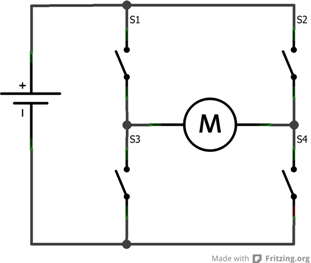
\includegraphics[width=4cm]{images/pontH1}
      \caption{\label{pontH1} Pont en H simple}
   \end{minipage}
   \begin{minipage}[c]{.33\linewidth}
      \centering
      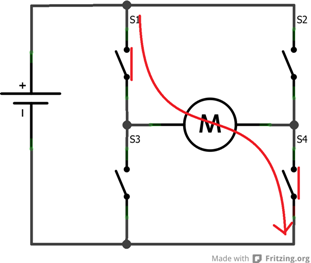
\includegraphics[width=4cm]{images/pontH2}
      \caption{\label{pontH2} Pont H sens 1}
   \end{minipage}
   \begin{minipage}[c]{.33\linewidth}
       \centering
       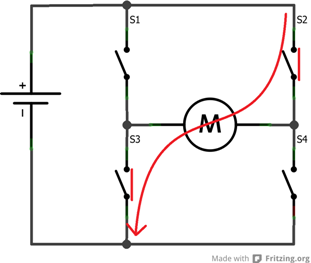
\includegraphics[width=4cm]{images/pontH3}
       \caption{\label{pontH3} Pont H sens2}
   \end{minipage}
\end{figure}

Dans la figure~\ref{pontH1} on retrouve un pont en H réaliser à partir de simple interrupteurs. Si
S1 et S4 (\ref{pontH2}) sont fermé en même temps le courant va parcourir le moteur dans un sens. Si S2
et S3 \ref{pontH3} sont fermé le courant va parcourir le moteur dans le sens inverse.

On peut aussi courcircuiter le moteur pour créer un phénomène de frein magnétique. Le moteur va
génerer être freiner par le courant qu'il va générer lui même. 

\begin{figure}[!h]
   \begin{minipage}[c]{.50\linewidth}
      \centering
      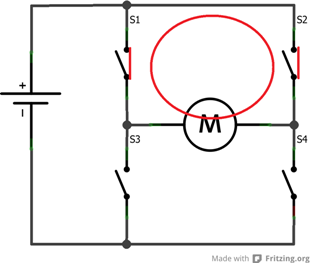
\includegraphics[width=4cm]{images/pontH4}
      \caption{\label{pontH4} Frein magnétique S1,S2}
   \end{minipage}
   \begin{minipage}[c]{.50\linewidth}
      \centering
      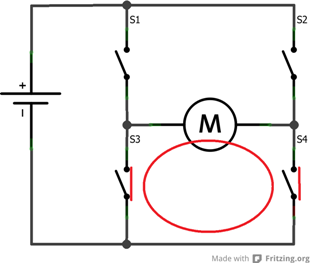
\includegraphics[width=4cm]{images/pontH5}
      \caption{\label{pontH5} Frein magnétique S3,S4}
   \end{minipage}
\end{figure}

Un pont En H réel n'est pas fait à partir d'interrupteur mais de transistor. Il faut savoir que
lorsque le moteur ne sera pas alimenté il va génerer un courant dit de "roue libre". Ce courant peut
abimer les transistors dans ce cas il faut le protéger pour cela on va utiliser des diodes de roues
libres.

\begin{figure}[!h]
   \centering
   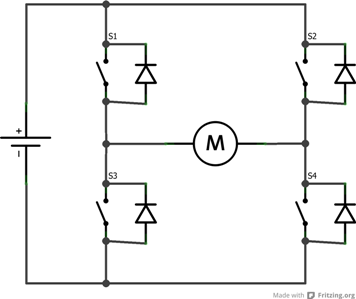
\includegraphics[width=4cm]{images/pontHDiodes}
   \caption{\label{pontH4} Diode de roue libre}
\end{figure}

Ainsi lorsque le moteur n'est pas alimenté le courant généré par le moteur passera dans les diodes
de roues libres	et non dans les transistors. Ce qui permet de les préserver.

\subsection{Conception Naive}

Afin de mieux apréhender le fonctionnement d'un pont en H j'ai réalisé un premier prototypes sans
utiliser un composant tout fait tel un L298

Ajouter photo proteus

À l'aide du logiciel de simulation Proteus et plusieurs prototype j'en suis arrivé au résultat
suivant : 

Puis j'ai réalisé ce prototype sur une petite carte en bakélite

Ajouter photo

\subsection{Conception d'un vrai Circuit de control Moteur}

\cite{MoteurCCEskimon}
\bibliographystyle{plain}
\bibliography{elec}

http://eskimon.fr/285-arduino-601-le-moteur-courant-continu
http://ancrobot.free.fr/Old_version/fichtech/action/ponth/index.htm
http://ancrobot.free.fr/Old_version/fichtech/action/ponthII/index.htm

\end{document}
